\directlua{pdf.setminorversion(4)}

\documentclass{standalone}
\usepackage{tikz}
\usepackage{tikz-feynman}

\begin{document}

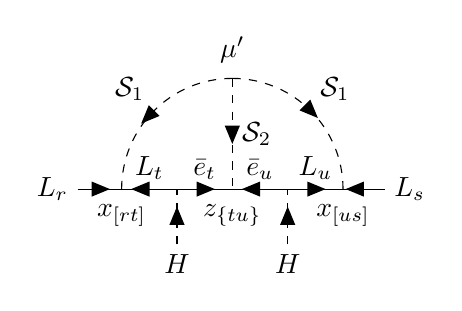
\begin{tikzpicture}
  \begin{feynman}
    \vertex (A) {$L_{r}$};
    \vertex [right=2.5em of A] (B);
    \vertex [below=0.2em of B] (Blabel) {$x_{[rt]}$};
    \vertex [right=2em of B] (CH);
    \vertex [below=2em of CH] (CHlabel) {$H$};
    \vertex [right=2em of CH] (C);
    \vertex [below=0.2em of C] (Clabel) {$z_{\{tu\}}$};
    \vertex [right=2em of C] (DH);
    \vertex [below=2em of DH] (DHlabel) {$H$};
    \vertex [right=2em of DH] (D);
    \vertex [below=0.2em of D] (Dlabel) {$x_{[us]}$};
    \vertex [right=1.5em of D] (E) {$L_{s}$};
    \vertex [above=4em of C] (F);
    \vertex [above=0.2em of F] (Flabel) {$\mu^{\prime}$};
    \diagram* {
      (A) -- [fermion] (B) -- [anti fermion, edge label=$L_{t}$] (CH) -- [fermion, edge label=$\bar{e}_{t}$] (C) -- [anti fermion, edge label=$\bar{e}_{u}$] (DH) -- [fermion, edge label=$L_u$] (D) -- [anti fermion] (E),
      (B) -- [anti charged scalar, quarter left, edge label=$\mathcal{S}_{1}$] (F) -- [charged scalar, quarter left, edge label=$\mathcal{S}_{1}$] (D),
      (F) -- [charged scalar, edge label=$\mathcal{S}_{2}$] (C),
      (CHlabel) -- [charged scalar] (CH),
      (DHlabel) -- [charged scalar] (DH),
    };
  \end{feynman}
\end{tikzpicture}

\end{document}
